\documentclass{article}
\usepackage[a4paper,margin=3.5cm,footskip=.5cm]{geometry}
\usepackage[utf8]{inputenc}
\usepackage{graphicx}
\usepackage{parskip}

\title{Architecture 2D-GC visualization}

\author{
  Baksteen, Sarah\\
  \texttt{S3145034}
  \and
  Brink, Wouter\\
  \texttt{S3862348}
  \and
  Gros, Oane\\
  \texttt{S2972778}
  \and
  Jager, Maarten de \\
  \texttt{S2957906}
  \and
  Jong, Michiel de \\
  \texttt{S2550768}
  \and
  Strik, Oliver\\
  \texttt{S3100693}
}
\date{}

\begin{document}
\clearpage
\maketitle
\thispagestyle{empty}
\begin{center}
    \vfill
    
\includegraphics[width=0.8\textwidth]{UG_logo.jpg}
    \vfill
    
    \Large
    \textbf{Client} \\
    Rohrbach, Léon \\
    Figueiredo, Monique \\
    
    \vspace{1cm}
    \textbf{TA} \\
    Argyrousis, George
    
    \vspace{2cm}
        Software Engineering \\
        University of Groningen \\
        \today \\
        \empty
        
        \vspace{1cm}
        Version 2.0
\end{center}

\newpage\setcounter{page}{1}
\subsection*{Introduction}

The product we are developing is a tool to be used for the visualization and processing of 2D-GC data. This data is obtained through the process of gas chromatography and can give insight in the specific compound being analyzed. To effectively perform the analysis of a certain compound the ability to visualize the data in multiple dimensions is required. As 3D and 2D visualization of the data is deemed to have priority over the 1D visualization, the latter will not be part of the product for now. In order to view the visualized data in greater detail the product allows for zooming and moving within a graph. In addition the product enables the labeling of peaks and the integration over selected data.

\section*{Architectural Overview}
The general architecture is based on the MVC-model where the architecture is divided into 3 main components. In the most general case of an MVC-architecture there exists a controller with which the user interacts, the controller consequently manipulates the model component according to the input given by the user. The model then updates the view, which in its turn is shown to the viewer. For this particular program the MVC-model is slightly modified and a broad representation is given by figure 1.\\

\begin{figure}[h]
    \centering
    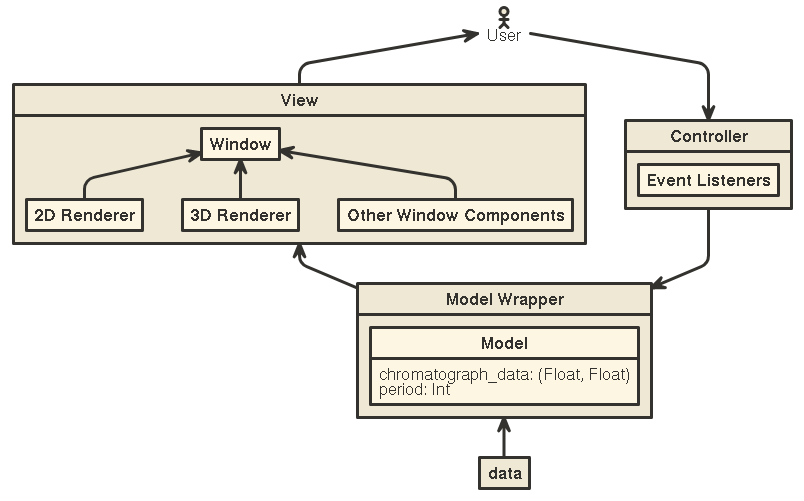
\includegraphics[scale=0.5]{nomnoml.png}
    \caption{Diagram representation of the MVC-model used}
    \label{fig:my_label}
\end{figure}
The view component represents what is shown by the program on the main window. As requested the main window contains a 3d-visualization of the gc data and a 2d visualization of the 2d-gc data alongside the 3d graph. For now the architecture does not include the 1d representation and most of the functionality to be included in the 'other window components' is not present yet. Functionality such as zooming and moving within the graph is handled by the libraries which generate the visualization of the data themselves. \\

The model wrapper contains the model, that is in this case, the data. Since the user needs to be able to save peak data and corresponding information on integration values and labels and such it is necessary for the model to be able to write files.\\

\section*{Technology Stack}
The product is build on Python 3 software, which due to it's many available libraries and packages concerning data visualization and manipulation, makes for an convenient implementation. The used libraries include:

\begin{itemize}
    \item \textbf{SciPy/NumPy} - SciPy and its sublibrary NumPy are used for advanced 2D data manipulation, such as the integration, convolution and other array operations. This library was chosen because it is an industry standard and very fast and easy in use. 
    \item \textbf{PyQtGraph} - PyQtGraph is used for the plotting of both the 2D and 3D data, and was chosen because it is an effective library for both 2D and 3D plotting of graphs, and has relatively good support for surface plots. The PyQtGraph package also contains some GUI elements, which it inherits from PyQt5, and the functionality for drawing and manipulating regions of interest, which we use for integration.
    \item \textbf{PyOpenGl} - Is a dependency of PyQtGraph and the industry standard for 3D graphics, we have chosen to work on the OpenGL functionality to accommodate more intuitive palette controls and coloring of the 3D graph.
    \item \textbf{PyQt5} - The PyQtGraph GUI is built on the PyQt5 library, this is why we have built the rest of the GUI on the same structure.
   %\item \textbf{PyQt5-sip} - Dependency of PyQt5 % What is this, and why do we name it?
\end{itemize}

\section*{Acronyms}

\textbf{2D-GC} Two Dimentional Gas Chromatography.
\textbf{MVC} Model View Controller.

\section*{Glossary}


\section*{Change Log}

\begin{tabular}{|c|c|c|}
     \hline
     Date& author & description \\
     \hline
     19-03-2019 & Maarten de Jager & initialized the document \\
     \hline
     01-04-2019 & Oliver Strik & Updated to respect the new Qt program \\
     \hline
     05/05/2019 & Oane Gros & Explained the choices in the technology stack \\
     \hline
\end{tabular}

\end{document}
